% chapter11.tex -- Maintaining the Valid Generating Set (VGS) and Implementation
% Based on the author's UGThesis.docx.

\chapter{Maintaining the Valid Generating Set (VGS) and Implementation}
\label{ch:vgs}

In this chapter we address the implementation details that allow us to flip generating chords in constant time while avoiding multi-edge conflicts. 
We introduce the \textbf{valid generating set} (VGS), a subset of the generating set containing only those chords whose flip is safe (i.e., does not create a multi-edge with previously added chords). 
We show how to initialise and update the VGS in constant time per flip, using linked lists and a global hash set for chord existence queries.

\section{The Problem of Checking Multi-Edge Before Flipping}
\label{sec:vgs_problem}

Recall from Chapter~\ref{ch:multi_layer_dfs} that when we are at a triangulation \(T\) of the current face, we only flip a generating chord \((v_r, v_j)\) if its opposite pair \((v_o, v_{o'})\) is not already present in the global chord set \(S\). 
This check requires a membership query in \(S\), which we can perform in expected \(O(1)\) time using a hash set.

However, after flipping a chord, the set of generating chords for the child triangulation changes, and some chords that were previously safe may become unsafe (or vice versa). 
We must update the set of candidate chords that can be flipped in the next steps without performing an expensive recomputation from scratch.

\section{Two Options}
\label{sec:vgs_options}

We have two possible approaches to maintain the set of flippable chords:

\begin{enumerate}[label=\textbf{Option \arabic*:}]
    \item \textbf{Maintain a valid generating set (VGS)} that contains exactly those generating chords whose flip is safe (i.e., the opposite pair is not in \(S\)). 
    Whenever we flip a chord, we update the VGS for the affected chords (at most four border chords) in constant time.
    
    \item \textbf{Prove that invalid checks do not affect total time.} 
    That is, we could check the opposite pair against \(S\) at the moment we consider flipping a chord, and if it is unsafe, we simply skip that child. 
    The cost of these checks would then be proportional to the number of generating chords considered, which could be larger than the number of flips performed. 
    However, we can bound the total number of checks by the total number of nodes in the genealogical tree, which is \(O(T)\) (where \(T\) is the number of triangulations). 
    This approach also works in theory, but it requires careful amortised analysis to ensure that the overhead of checking chords that are never flipped is not too large.
\end{enumerate}

We choose \textbf{Option 1} because it yields a clean constant-time bound per flip and avoids any additional amortised argument. 
The VGS approach was described in the original thesis and is implemented as follows.

\section{Definition of the Valid Generating Set (VGS)}
\label{sec:vgs_definition}

\begin{definition}[Valid generating set]
    \label{def:vgs}
    Let \(T\) be a triangulation of a face with root vertex \(v_r\). 
    The \textbf{valid generating set} \(VGS\) is the set of all generating chords \((v_r, v_j)\) of \(T\) (i.e., chords with \(j \ge b'\), where \((v_b, v_{b'})\) is the leftmost blocking chord of \(T\)) such that the opposite pair \((v_o, v_{o'})\) is \emph{not} present in the global chord set \(S\).
\end{definition}

Initially, when we build the root triangulation from a safe root, all generating chords are valid because by definition of a safe root, none of the chords \((v_r, v_j)\) belongs to \(S\), and for the root triangulation the opposite pairs are chords that do not have \(v_r\) as an endpoint; they are new chords not yet in \(S\) (since the face is processed for the first time). 
Thus the initial VGS is identical to the generating set \(GS\).

\section{How Flipping Affects Border Chords}
\label{sec:vgs_flip_effect}

When we flip a generating chord \((v_r, v_j)\), the operation affects only the four chords that form the boundary of the quadrilateral in which the flip occurs. 
Consider the quadrilateral \((v_r, v_a, v_j, v_b)\) in clockwise order, where \((v_a, v_b)\) is the opposite pair of \((v_r, v_j)\). 
Flipping removes \((v_r, v_j)\) and adds \((v_a, v_b)\). 
The chords that change their opposite pairs are the two chords incident to \(v_r\) that are adjacent to \((v_r, v_j)\) in the cyclic order, namely \((v_r, v_a)\) and \((v_r, v_b)\) (if they exist and are generating chords), and also the two chords that share the quadrilateral boundaries? 
A careful analysis from the original paper shows that at most four chords have their opposite pairs updated: the two neighbours of \((v_r, v_j)\) on the left and right, and the two chords that become adjacent to the new diagonal.

In practice, the only chords whose status in VGS may change are the two generating chords adjacent to \((v_r, v_j)\) in the clockwise order around \(v_r\). 
The other two border chords are not generating (they do not have \(v_r\) as an endpoint) and are irrelevant for VGS. 
Thus each flip affects at most two chords in the VGS.

\begin{figure}[htbp]
    \centering
    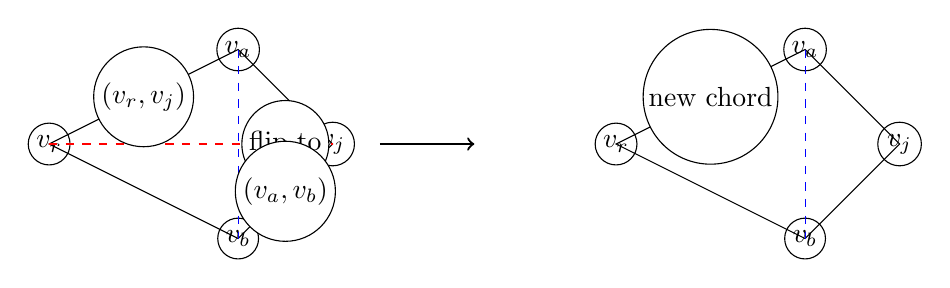
\begin{tikzpicture}[scale=1.2, every node/.style={circle, draw, fill=white, inner sep=1.5pt}]
        \coordinate (R) at (0,0);
        \coordinate (A) at (2,1);
        \coordinate (J) at (3,0);
        \coordinate (B) at (2,-1);
        \node at (R) {\(v_r\)};
        \node at (A) {\(v_a\)};
        \node at (J) {\(v_j\)};
        \node at (B) {\(v_b\)};
        \draw (R)--(A)--(J)--(B)--cycle;
        \draw[dashed, red] (R)--(J);
        \draw[dashed, blue] (A)--(B);
        \node at (1,0.5) {\((v_r, v_j)\)};
        \node at (2.5,0) {flip to};
        \node at (2.5,-0.5) {\((v_a, v_b)\)};
        \draw[->, thick] (3.5,0) -- (4.5,0);
        \begin{scope}[xshift=6cm]
            \coordinate (R2) at (0,0);
            \coordinate (A2) at (2,1);
            \coordinate (J2) at (3,0);
            \coordinate (B2) at (2,-1);
            \node at (R2) {\(v_r\)};
            \node at (A2) {\(v_a\)};
            \node at (J2) {\(v_j\)};
            \node at (B2) {\(v_b\)};
            \draw (R2)--(A2)--(J2)--(B2)--cycle;
            \draw[dashed, blue] (A2)--(B2);
            \node at (1,0.5) {new chord};
        \end{scope}
    \end{tikzpicture}
    \caption{Flipping a generating chord \((v_r, v_j)\) in quadrilateral \((v_r, v_a, v_j, v_b)\). 
    The opposite pairs of the chords \((v_r, v_a)\) and \((v_r, v_b)\) may change, affecting their membership in the VGS.}
    \label{fig:flip_affects_border}
\end{figure}

\section{Four Possible Situations for Border Chords}
\label{sec:vgs_four_cases}

Let \((v_r, v_a)\) be a neighbouring generating chord of \((v_r, v_j)\). 
Before the flip, it has an opposite pair \((v_x, v_y)\). 
After the flip, its opposite pair may change to \((v_x', v_y')\). 
Depending on whether the chord was in VGS before and whether the new opposite pair is in \(S\), we have four cases:

\begin{enumerate}
    \item \textbf{Was safe, becomes unsafe.} 
    The chord was in VGS, but after the flip its new opposite pair is already in \(S\). 
    We remove it from VGS.
    
    \item \textbf{Was unsafe, becomes safe.} 
    The chord was not in VGS (its old opposite pair was in \(S\)), but after the flip the new opposite pair is not in \(S\). 
    We add it to VGS.
    
    \item \textbf{Was safe, remains safe.} 
    No change.
    
    \item \textbf{Was unsafe, remains unsafe.} 
    No change.
\end{enumerate}

Since at most two border chords are affected, we can update the VGS in constant time by checking the new opposite pair against \(S\) (a hash set lookup) and inserting or removing the chord from the VGS list.

\section{Constant-Time Operations Using Linked Lists}
\label{sec:vgs_linked_lists}

We implement the VGS as a doubly linked list. 
Each node in the list corresponds to a generating chord \((v_r, v_j)\) and stores:
\begin{itemize}
    \item The endpoint \(j\) (or a pointer to the vertex).
    \item A pointer to the opposite pair \((v_o, v_{o'})\).
    \item Pointers to the previous and next elements in the VGS list.
\end{itemize}
Additionally, we maintain an array or hash map from the chord identifier (e.g., the index \(j\)) to its list node, so that we can remove or add a chord in \(O(1)\) time given its index.

When we flip a chord \((v_r, v_j)\), we:
\begin{enumerate}
    \item Remove \((v_r, v_j)\) from the VGS (if it was in VGS — by definition it is, because we only flip chords from VGS).
    \item Update the opposite pairs of the two neighbouring generating chords (say \((v_r, v_a)\) and \((v_r, v_b)\)) by recomputing their opposite pairs from the new triangulation.
    \item For each of these two chords, check whether the new opposite pair is in \(S\). 
    If it is not in \(S\) and the chord is not already in VGS, add it to VGS. 
    If it is in \(S\) and the chord is currently in VGS, remove it from VGS.
\end{enumerate}

All these operations take \(O(1)\) time.

\section{Initialising the VGS During Root Triangulation Building}
\label{sec:vgs_initialisation}

When we construct a safe root triangulation for a face, we:
\begin{enumerate}
    \item Compute the safe root \(v_r\) using the two-pointer algorithm (Chapter~\ref{ch:safe_root_algorithm}).
    \item Add all chords \((v_r, v_j)\) for \(j = r+2, r+3, \dots, r-2\) (mod \(n\)).
    \item For each such chord, compute its opposite pair \((v_{j-1}, v_{j+1})\) (indices modulo \(n\)).
    \item Check whether the opposite pair is already in \(S\). 
    By definition of a safe root, none of the chords \((v_r, v_j)\) is in \(S\), but the opposite pairs may or may not be in \(S\). 
    However, recall that \(S\) contains chords from previous faces, which lie outside the current face. 
    Could an opposite pair \((v_{j-1}, v_{j+1})\) be already in \(S\)? 
    It is possible if that chord was added when triangulating a previous face that shares the edge \((v_{j-1}, v_{j+1})\) as a chord. 
    In that case, the generating chord \((v_r, v_j)\) would be unsafe from the start, and we should not include it in VGS. 
    Indeed, the definition of a safe root only guarantees that the chords from \(v_r\) to non-neighbours are not in \(S\); it does not guarantee anything about opposite pairs. 
    Therefore, during initialisation we must compute the VGS as the subset of generating chords whose opposite pair is not in \(S\).
\end{enumerate}

Thus the initial VGS may be smaller than the full generating set. 
This is fine; the root triangulation itself is still valid (since all its chords are safe), but some generating chords may be unsafe to flip immediately. 
They will never become safe later because flipping other chords does not change the opposite pair of a chord that is not adjacent to the flip? 
Actually, the opposite pair of a generating chord can change when a neighbouring generating chord is flipped (as described above). 
So a chord that is initially unsafe may become safe later. 
This is handled by the dynamic updates.

\section{Global Hash Map for Chord Existence}
\label{sec:vgs_hashmap}

We maintain a global hash set \(S\) (or hash map) that stores all chords that have been permanently added from previous faces and from the current partial triangulation along the DFS path. 
The hash set supports three operations in expected \(O(1)\) time:
\begin{itemize}
    \item \texttt{insert(chord)} – add a chord to \(S\).
    \item \texttt{remove(chord)} – remove a chord from \(S\) (used during backtracking).
    \item \texttt{contains(chord)} – test whether a chord is already in \(S\).
\end{itemize}

Chords are represented as unordered pairs \((a, b)\) with \(a < b\). 
To avoid collisions, we use a standard hash function (e.g., \((a \cdot n + b)\) modulo a prime). 
The total number of chords stored in \(S\) at any time is \(O(n)\) because the partial triangulation of a planar graph with \(n\) vertices has at most \(3n-6\) edges (by Euler’s formula). 
Thus the hash set uses \(O(n)\) space.

\section{Implementation Summary}
\label{sec:vgs_implementation_summary}

The following data structures are used for each face during its local DFS:
\begin{itemize}
    \item \texttt{List L}: all chords of the current triangulation (stored as pairs).
    \item \texttt{List GS}: all chords incident to the root vertex (generating set, unfiltered).
    \item \texttt{List VGS}: subset of GS that are currently safe to flip.
    \item \texttt{Array opposite}: for each generating chord \((v_r, v_j)\), store its opposite pair \((v_o, v_{o'})\).
    \item \texttt{HashMap chordToNode}: mapping from chord \((v_r, v_j)\) to its node in the VGS list for constant-time removal.
\end{itemize}

The global hash set \(S\) is shared across all faces and is updated with push/pop operations during recursion.

\section{Correctness of the VGS Maintenance}
\label{sec:vgs_correctness}

We claim that the VGS always contains exactly those generating chords whose flip would produce a child that does not immediately create a multi-edge (i.e., the opposite pair is not in \(S\)). 
Moreover, when we flip a chord from VGS, the child triangulation is guaranteed to be valid (its chords are all either from the parent or the new chord, and the new chord is not in \(S\) by construction). 
After the flip, we update the VGS for the affected chords, preserving the invariant for the child.

Thus the algorithm never attempts to flip an unsafe chord, and all generated triangulations are free of multi-edges.

\section{Summary}
\label{sec:vgs_summary}

We have introduced the valid generating set (VGS) as a dynamic subset of the generating set containing only those chords whose flip is safe. 
By maintaining the VGS as a linked list and updating at most two chords per flip, we achieve constant-time updates. 
The global hash set \(S\) provides expected \(O(1)\) membership queries. 
These data structures together enable our algorithm to generate all valid triangulations in \(O(1)\) amortised time per triangulation.